\chapter{Giới thiệu các công nghệ đã sử dụng}


\section{Phát triển trang web}

Phát triển trang web là một quá trình tạo ra các ứng dụng hay trang web có thể chạy trên các trình duyệt web. Quá trình này bao gồm nhiều giai đoạn khác nhau từ việc thiết kế giao diện người dùng (UI) đến việc thiết kế cơ sở dữ liệu (back-end).

Phát triển trang web cần đòi hỏi chúng ta phải nắm vững được những chức năng, đặc điểm của trang web. Ngoài những chức năng, đặc điểm nổi bật, còn có những thách thức tiềm ẩn khác đối với các nhà phát triển cho trang web, như là:

\begin{itemize}
    \item Hiệu suất: Với việc cung cấp một trải nghiệm tốt cho người dùng, việc đo lường hiệu suất sẽ giúp cho các nhà phát triển có thể hiểu rõ được các yếu tố có thể ảnh hưởng đến phần mềm. Và việc cải thiện chúng là 1 vấn đề không hề dễ đối với các nhà phát triển.
    \item Bảo dưỡng, bảo trì, cập nhật: Vấn đề về cập nhật và bảo trì dữ liệu sẽ là một trở ngại với các nhà phát triển nếu việc tổ chức, sắp xếp các dữ liệu không được tốt.
    \item Lưu lượng kết nối, tốc độ tải trang: Cũng giống như việc bảo dưỡng, bảo trì thì nếu các dữ liệu được tổ chức một cách lộn xộn, không nhất quán thì sẽ ảnh hưởng đến tốc độ tải trang của trang web và làm ảnh hưởng đến lưu lượng kết nối và gây tắc nghẽn mạng.
\end{itemize}

\section{Phát triển front-end}
Phát triển front-end là quá trình tạo ra giao diện của người dùng của một ứng dụng hoặc trang web. Đây là một quy trình xây dựng giao diện người dùng (UI) và trải nghiệm của người dùng (UX) của một trang web. Đây là phần "mặt tiền" của sản phẩm số, nơi người dùng có thể tương tác trực tiếp với các yếu tố hiển thị trên màn hình như: văn bản, hình ảnh, nút bấm,.... Đây là thứ mà người dùng sẽ dành một lượng lớn thời gian để tương tác. Do đó, mục tiêu chính của việc phát triển front-end là tạo ra giao diện thân thiện với người dùng, hấp dẫn và dễ sử dụng, đồng thời bảo đảm tính tương tác và tốc độ tải trang tối ưu.

Với việc thế giới công nghệ ngày càng bao trùm xung quanh ta, việc thích nghi với chúng là không thể tránh khỏi. Trang web này được thiết kế để giúp cho người sắp và đang đi làm trong việc hỗ trợ người dùng viết một bản CV hoàn chỉnh, đẹp mắt và giúp tạo điểm nhấn với các nhà tuyển dụng. Bên cạnh đó, trang web cũng đồng thời giúp người dùng tìm kiếm công việc ngay trên trang web với bản CV mà người dùng đã hoàn thiện.

Ngày xưa, việc đăng tuyển việc làm và tìm kiếm nhân tài cho công ty là 1 vấn đề nan giải với các nhà tuyển dụng. Đồng thời, những người tìm việc cũng phải "ngụp lặn" với những thứ bòng bong từ những thông tin đa chiều từ nhiều trang báo khác nhau. Thì giờ nay, chỉ với một chiếc điện thoại, ai cũng có thể đăng tuyển hay nộp đơn xin việc một cách rất dễ dàng. Và những thông tin đăng tuyển rất đa dạng từ mọi ngành nghề đến những ngôn ngữ khác nhau. Bên cạnh đó, CV cũng có những template (mẫu) rất đa dạng phù hợp với mọi ngành nghề, đồng thời, người dùng cũng có thể tự mình thiết kế cho mình những bản CV theo ý thích của mình.

Dưới đây là những công nghệ được sử dụng trong đồ án lần này:

\subsection{ReactJS}
React (ReactJS) là một thư viện JavaScript mã nguồn mở, được dùng để xây dựng giao diện người dùng (front-end) cho web. React chỉ tập trung vào phần hiển thị giao diện, chứ không can thiệp vào cách sắp xếp logic nghiệp vụ hoặc cấu trúc ứng dụng.

React tập trung vào việc hiển thị giao diện và cho phép lập trình viên tự do quyết định cách sắp xếp logic nghiệp vụ. Chính sự linh hoạt này làm cho React trở nên phổ biến, vì nó phù hợp với nhiều loại dự án và phong cách phát triển khác nhau. Khác với các framework có kiến trúc cố định như Angular, React không ép buộc người dùng vào một mô hình cụ thể khiến nó linh hoạt rất nhiều cho nhiều dự án khác nhau.

React được xây dựng dựa trên kiến trúc component, nơi mỗi thành phần có thể được tái sử dụng giúp ứng dụng dễ mở rộng và duy trì. Điều này giúp các lập trình viên dễ dàng phát triển các ứng dụng lớn hơn bằng cách chia nhỏ các thành phần độc lập, có thể tái sử dụng mà không cần phải lo về việc tích hợp phức tạp.

Dưới đây là một số component chính của ReactJS được sử dụng trong đề tài này:

\subsubsection{Virtual DOM}
\textbf{Virtual DOM} (Document Object Model ảo) là một bản sao nhẹ hơn của DOM thật. DOM thật là cấu trúc cây chứa tất cả các thành phần HTML trong trang web. Và khi người dùng tương tác với ứng dụng thì ứng dụng sẽ thay đổi và DOM thật cũng được cập nhật.

\begin{figure}[htp!]
    \centering
    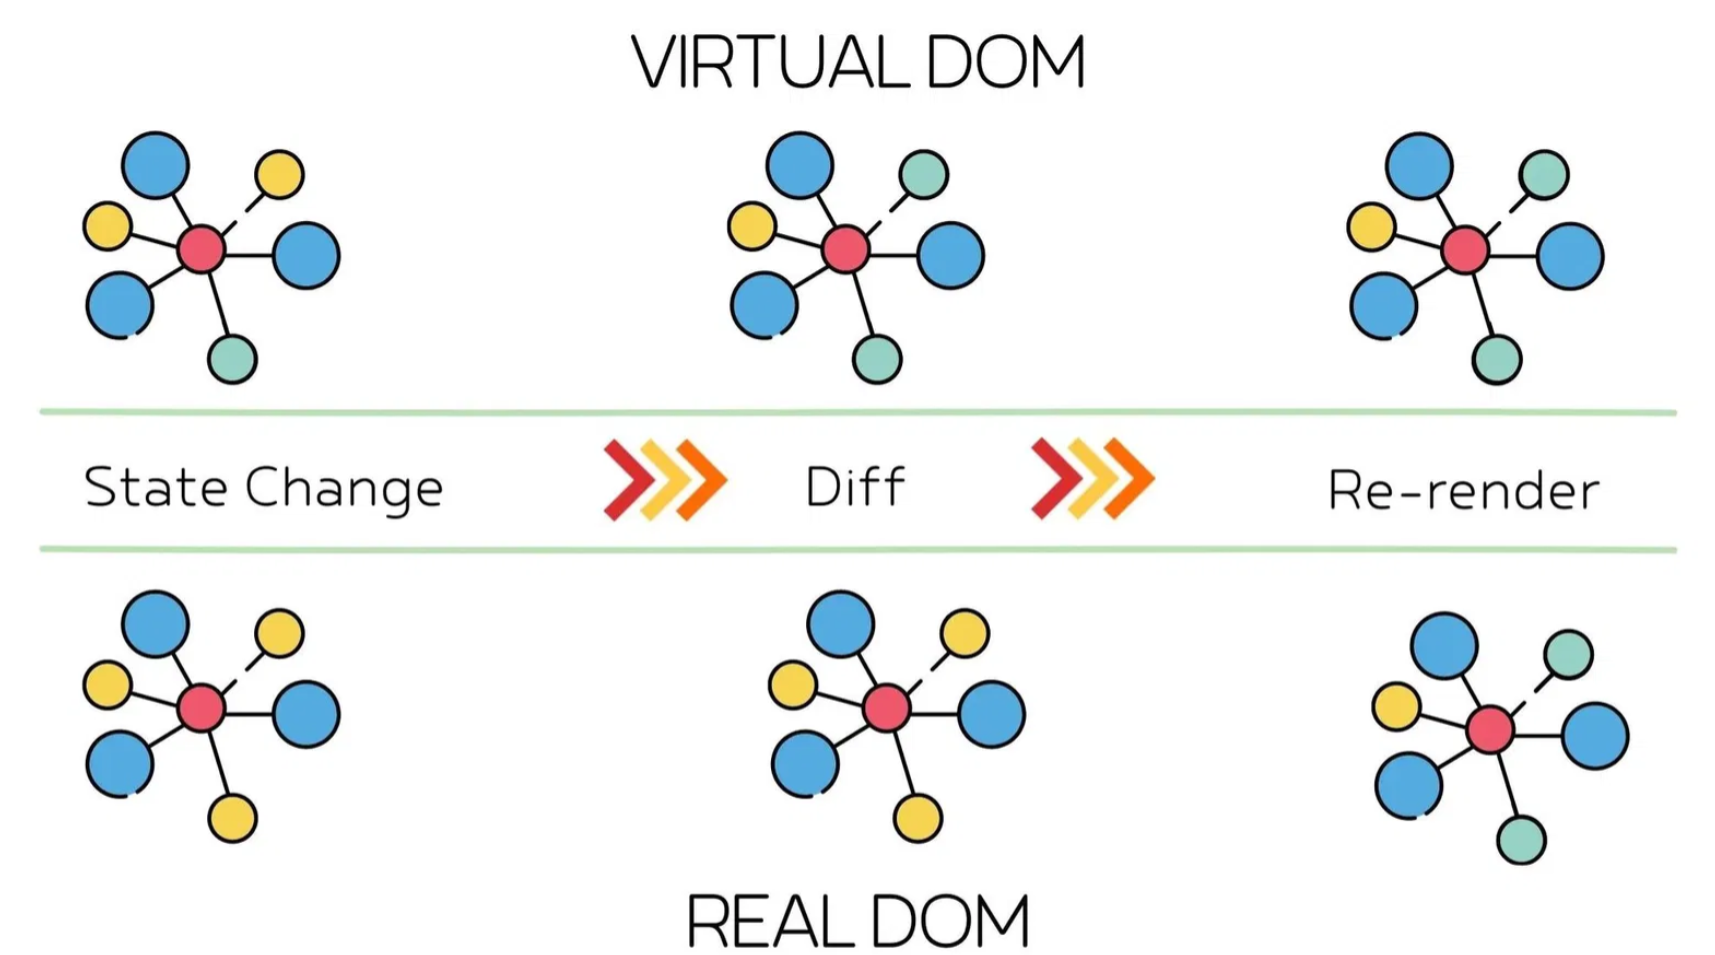
\includegraphics[scale=0.35]{img/Virtual-DOM.png}
    \caption{So sánh giữa DOM ảo (Virtual DOM) và DOM thật (Real DOM)}
    \label{fig:virtualDOM}
\end{figure}

Tuy nhiên, việc cập nhật DOM thật có thể gây ra tình trạng chậm chạp và kém hiệu quả đặc biệt là ở trong các ứng dụng lớn với nhiều phần tử. Vì vậy, React đã sử dụng DOM ảo với mục đích chỉ những phần có sự thay đổi mới được cập nhật lên DOM thật giúp tiết kiệm thời gian và tài nguyên.

\subsubsection{Redux Toolkit}
Đầu tiên, Redux là một thư viện quản lý trạng thái tương thích với các ứng dụng web. Đây là một công cụ hữu ích giúp bạn xây dựng các ứng dụng có tính nhất quán, hoạt động linh hoạt trên nhiều môi trường (client, server và native), và dễ dàng kiểm thử. Do sáng tạo từ ngôn ngữ Elm và kiến trúc Flux của Facebook,  do đó, Redux thường được kết hợp sử dụng cùng với React.

Redux có nhiệm vụ quản lý trạng thái phức trong ứng dụng web, giúp tách biệt logic và giao diện người dùng. Với việc tiếp cận dễ hiểu và dễ theo dõi, Redux sẽ giúp bạn theo dõi và cập nhật trạng thái một cách hiệu quả, đồng thời đảm bảo tính nhất quán của dữ liệu trong ứng dụng.

Tuy nhiên, một số lập trình viên cảm thấy Redux hơi dài dòng và khó sử dụng. Với những bất cập như việc tạo một store hoàn chỉnh cần đòi hỏi nhiều bước và tạo nhiều tệp lặp đi lặp lại. Nhằm tối giản hóa cách setup và sử dụng, Redux Toolkit được ra đời. Nó giúp các lập trình viên có thể tập trung hơn vào việc xử lý logic thay vì mất quá nhiều thời gian ban đầu để setup.

Redux Toolkit là một thư viện được phát triển bởi ReduxJS, giúp việc viết mã Redux nhanh chóng và toàn diện. Nó giải quyết vấn đề phức tạp của Redux và cung cấp API tiện ích để viết mã ngắn gọn, dễ đọc hơn. Ngoài ra, Redux Toolkit còn có nhiều lợi ích khác bên cạnh:

\begin{itemize}
    \item \textbf{Đơn giản hoá quy trình phát triển}: Redux Toolkit giúp giảm số lượng mã cần phải viết và đơn giản hoá các cú pháp. Điều này không chỉ giúp tiết kiệm thời gian mà còn làm cho mã nguồn trở nên dễ đọc và bảo trì tốt hơn.
    \item \textbf{Giảm thiểu mã lặp lại}: Một trong những vấn đề lớn khi sử dụng Redux là mã lặp lại. Redux Toolkit cung cấp các utility functions giúp bạn tạo ra reducers và actions một cách nhanh chóng và hiệu quả.
    \item \textbf{Hỗ trợ cho các tác vụ bất đồng bộ}: Redux Toolkit tích hợp sẵn các công cụ để xử lý các tác vụ bất đồng bộ thông qua createAsyncThunk. Điều này giúp bạn dễ dàng quản lý các yêu cầu API mà không cần phải viết nhiều mã phức tạp để xử lý trạng thái loading và error.
    \item \textbf{Tích hợp dễ dàng với React}: Redux Toolkit được thiết kế để hoạt động tốt với React, cung cấp các API như configureStore để dễ dàng cấu hình store và kết nối với các component. Điều này giúp bạn nhanh chóng tích hợp Redux vào ứng dụng React mà không gặp phải nhiều khó khăn.
    \item \textbf{Tăng cường hiệu suất}: Việc sử dụng Redux Toolkit giúp chuẩn hóa dữ liệu trước khi lưu vào Redux store, từ đó cải thiện hiệu suất của ứng dụng. Điều này đặc biệt quan trọng trong các ứng dụng lớn với nhiều state phức tạp.
\end{itemize}

\subsection{Vite}
Vite là một công cụ build và phát triển ứng dụng web được tạo ra bởi Evan You, người đã phát triển Vue.js, Vite ra đời mục đích khắc phục những hạn chế về tốc độ và hiệu suất. Nó cung cấp một cách tiếp cận mới để xây dựng các dự án web bằng cách tận dụng các mô-đun ES gốc trong trình duyệt và cung cấp tính năng thay thế mô-đun nóng (HMR) nhanh chóng. Tính năng này cho phép cập nhật tức thì mà không cần tải lại trang hoặc làm mất trạng thái ứng dụng, giúp quá trình phát triển hiệu quả hơn.

Các tính năng chính của Vite bao gồm:
\begin{itemize}
    \item \textbf{Tệp theo yêu cầu được phân phát qua ESM (Mô-đun ECMAScript) gốc}: giúp loại bỏ nhu cầu đóng gói. Tính năng này cải thiện đáng kể tốc độ và hiệu suất của các dự án phát triển web.
    \item \textbf{Thay thế mô-đun nóng (HMR)}: một tính năng cho phép các nhà phát triển thực hiện các thay đổi đối với mã của họ và xem kết quả ngay lập tức mà không cần phải tải lại toàn bộ trang. Điều này không chỉ tăng tốc quá trình phát triển mà còn nâng cao trải nghiệm người dùng bằng cách duy trì trạng thái ứng dụng.
    \item \textbf{Cung cấp API plugin và API JavaScript}: cho phép các nhà phát triển tùy chỉnh và mở rộng các chức năng của nó theo yêu cầu của dự án của họ. Tính linh hoạt này làm cho Vite.js trở thành một công cụ linh hoạt cho nhiều dự án phát triển web.
\end{itemize}

\subsubsection{So sánh giữa Webpack và Vite}
\begin{table}[H]
    \centering
    \begin{tabular}{|>{\centering\arraybackslash}p{0.18\linewidth}|>{\centering\arraybackslash}p{0.35\linewidth}|>{\centering\arraybackslash}p{0.35\linewidth}|} \hline 
         &  Vite& Webpack\\ \hline 
         Tốc độ khởi động&  	Khởi động nhanh nhờ sử dụng ES Modules gốc của trình duyệt, chỉ tải các tệp cần thiết.& Khởi động chậm hơn do phải đóng gói toàn bộ mã trước khi chạy.\\ \hline 
         Phản hồi khi thay đổi mã&  HMR (Hot Module Replacement) nhanh, mượt mà, chỉ cập nhật phần code thay đổi.& HMR khả dụng nhưng có thể chậm hơn, đặc biệt với mã nguồn phức tạp.
\\ \hline 
         Cấu hình&  Cấu hình đơn giản, thân thiện với người mới bắt đầu, có sẵn thiết lập cho các framework phổ biến.	& Cấu hình phức tạp, cần nhiều thiết lập thủ công để tối ưu.
\\ \hline 
         Hỗ trợ mở rộng và plugin&  Hỗ trợ API plugin mạnh mẽ, dễ tùy chỉnh và mở rộng theo nhu cầu dự án.& Plugin hỗ trợ mạnh mẽ nhưng có thể phức tạp và khó tích hợp hơn.
\\ \hline 
         Kích thước build cuối cùng&  Dùng Rollup để đóng gói, thường tạo ra các file nhỏ gọn và tối ưu.& Có thể tối ưu kích thước build nhưng cần nhiều cấu hình để đạt hiệu quả tốt nhất.
\\ \hline
    \end{tabular}
    \caption{Bảng so sánh giữa Webpack và Vite}
    \label{tab:Vite}
\end{table}

\subsection{Axios}
Axios là thư viện giúp client tương tác với server thông qua giao thức HTTP dựa trên các Promises, có thể chạy được trên cả trình duyệt và NodeJS (phía server). Về cơ bản, nó cung cấp một API cho việc xử lý XHR (XMLHttpRequests). Ở phía trình duyệt, Axios sử dụng XMLHttpRequest (XHR) cung cấp một API cho việc gọi và xử lý request/response lên server; ngược lại ở phía server thì Axios sử dụng native module http trong NodeJS để xử lý.

Promise API được hiểu là một tập hợp các phương thức và tính năng liên quan đến Promises trong JavaScript. Promises là một cơ chế xử lý bất đồng bộ được sử dụng để xử lý các hoạt động mà cần thời gian để hoàn thành, chẳng hạn như các yêu cầu HTTP, đọc/ghi vào tệp, hoặc tương tác với cơ sở dữ liệu.

Trong phần cấu hình Axios, Axios cung cấp sẵn cho chúng ta 2 lựa chọn để chuyển đổi dữ liệu:

\begin{itemize}
    \item \textbf{TransformResponse}: cho phép bạn chuyển đổi dữ liệu từ response trước khi nó được trả về cho bạn.
    \item \textbf{TransformRequest}: cho phép bạn chuyển đổi dữ liệu trước khi gửi nó đi.
\end{itemize}

Ngoài ra, Axios còn có một tính năng mạnh mẽ gọi là Interceptors. Nó cho phép bạn can thiệp vào quy trình gửi và tiếp nhận yêu cầu HTTP trước và sau khi chúng được gửi. Bạn có thể sử dụng Interceptors để thực hiện các tác vụ như thêm tiêu đề, xử lý lỗi, thêm hoặc xoá thông tin từ yêu cầu và phản hồi, và nhiều tác vụ khác.
Axios cũng có hỗ trợ hai loại Interceptor chính:
\begin{itemize}
    \item \textbf{Request Interceptors}: Được gọi trước khi yêu cầu được gửi đi. Bạn có thể sử dụng chúng để thêm tiêu đề, thêm token xác thực, hoặc xử lý dữ liệu yêu cầu trước khi nó được gửi.
    \item \textbf{Response Interceptors}: Được gọi sau khi yêu cầu đã được gửi và phản hồi đã được nhận. Bạn có thể sử dụng chúng để xử lý dữ liệu phản hồi, xử lý lỗi, và thực hiện các tác vụ khác trên phản hồi.
\end{itemize}
 
Lý do sử dụng Axios:
\begin{itemize}
    \item \textbf{Dễ sử dụng và bảo trì}: Axios cung cấp một cách gọi API dễ đọc và dễ sử dụng hơn so với việc sử dụng XMLHttpRequest. Cú pháp của Axios rõ ràng và giúp tạo ra những đoạn code dễ bảo trì hơn về sau.
    \item \textbf{Hỗ trợ Promise}: Axios sử dụng Promise, giúp bạn quản lý bất đồng bộ dễ dàng hơn. Bạn có thể sử dụng .then() và .catch() để xử lý phản hồi và lỗi.
    \item \textbf{Hỗ trợ Interceptor}: Axios cho phép bạn sử dụng interceptors để can thiệp vào quy trình gửi và nhận yêu cầu HTTP, điều này giúp bạn thực hiện các tác vụ như thêm tiêu đề, xử lý lỗi, và nhiều tác vụ khác một cách dễ dàng.
    \item \textbf{Hỗ trợ tự động chuyển đổi dữ liệu}: Axios cho phép bạn tự động chuyển đổi dữ liệu từ JSON, XML và nhiều định dạng khác thành các kiểu dữ liệu JavaScript phổ biến như đối tượng hoặc mảng.
    \item \textbf{Hỗ trợ huỷ yêu cầu}: Axios cung cấp tích hợp hỗ trợ hủy yêu cầu, cho phép bạn hủy các yêu cầu đang chờ khi không còn cần thiết, ngăn cản các yêu cầu không mong muốn.
    \item \textbf{Hỗ trợ Xác thực}: Axios dễ dàng tích hợp với các phương thức xác thực khác nhau, bao gồm xác thực cơ bản, mã thông báo Bearer, và nhiều hình thức xác thực khác.
    \item \textbf{Hỗ trợ gửi yêu cầu CORS}: Axios mặc định đã tích hợp sẵn hỗ trợ gửi yêu cầu qua CORS (Cross-Origin Resource Sharing) và cho phép bạn tùy chỉnh các tiêu đề CORS dễ dàng.
    \item \textbf{Khả năng tuỳ chỉnh cao}: Axios có tính tùy chỉnh cao, cho phép bạn cấu hình nhiều khía cạnh của quy trình gửi và nhận yêu cầu HTTP.
    \item \textbf{Thư viện phổ biến và cộng đồng lớn}: Axios là một thư viện phổ biến và được sử dụng rộng rãi trong cộng đồng phát triển, điều này có nghĩa bạn có thể tìm thấy nhiều tài liệu hữu ích và hỗ trợ từ cộng đồng.
\end{itemize}

\subsection{TailwindCSS}
TailwindCSS là một framework CSS utility-first giúp tạo kiểu nhanh chóng và hiệu quả cho website mà không cần viết CSS thủ công. Thay vì cung cấp các thành phần (component) hoặc kiểu thiết kế mặc định, Tailwind cung cấp một loạt các lớp tiện ích (utility classes) mà bạn có thể kết hợp linh hoạt để xây dựng giao diện tùy chỉnh.

Tailwind cung cấp một bộ các lớp CSS được đặt tên theo chức năng của chúng, cho phép bạn kiểm soát trực tiếp các khía cạnh như bố cục, màu sắc, khoảng cách, kiểu chữ và bóng đổ mà không cần viết CSS tùy chỉnh. 

TailwindCSS hoạt động tốt nhất khi bạn muốn sáng tạo và kiểm soát thiết kế trang web của mình. Nó đặc biệt hữu ích cho các thiết kế độc đáo, các tính năng tương tác và các dự án mà giao diện là điểm quan trọng nhất. 

Ưu điểm của TailwindCSS:
\begin{itemize}
    \item \textbf{Giảm thiểu viết CSS tuỳ chỉnh}: Bạn có thể chỉnh sửa style của các thành phần bằng cách áp dụng những class được xây dựng sẵn vào HTML. Bằng cách này, bạn có thể xây dựng các thiết kế tuỳ chỉnh mà không cần viết CSS.
    \item \textbf{Giữ cho file CSS gọn nhẹ}: Với những class được xây dựng sẵn dưới dạng component như vậy, hầu hết các style đều có thể được tái sử dụng.
    \item \textbf{Thay đổi an toàn}: Với cách tiếp cận truyền thống, nếu bạn thay đổi CSS rất có thể một phần nào đó trên trang web sẽ bị lỗi. Tuy nhiên với Tailwind, các lớp tiện ích trong HTML là cục bộ, nhờ đó mà bạn không làm thay đổi những phần khác trên trang web. 
    \item \textbf{Tính đáp ứng và bảo mật}: Với các lớp dựng sẵn của Tailwind, bạn có thể thiết kế bố cục trực tiếp trong một file HTML. Điều này biến Tailwind thành một framework CSS đáp ứng cao, thân thiện với thiết bị di động. 
    \item \textbf{Xây dựng các ứng dụng web có khả năng đáp ứng}: Tailwind CSS bao gồm các lớp tích hợp sẵn để tạo các giao diện đáp ứng. Bạn không cần phải viết thêm CSS để điều chỉnh giao diện cho các thiết bị khác nhau. 
    \item \textbf{Tương thích với các thư viện JavaScript phổ biến}: Tailwind CSS tương thích với các thư viện JavaScript phổ biến như React, Vue.js và Angular.
    \item \textbf{Kiểm soát hoàn toàn đối với giao diện người dùng}: Tailwind CSS cung cấp cho bạn sự linh hoạt cao để tạo giao diện tùy chỉnh theo ý muốn. Bạn không bị giới hạn bởi các thành phần được thiết kế sẵn như trong các framework CSS khác. 
\end{itemize}

Nhược điểm của TailwindCSS:
\begin{itemize}
    \item \textbf{Quá trình đánh dấu (markup) trở nên dài dòng}: Không giống như các framework CSS khác, Tailwind hoạt động bằng cách trộn lẫn các quy tắc kiểu dáng trực tiếp vào các file HTML. Mặc dù điều này có lợi cho những người không quen thuộc với CSS nhưng nó cũng đi ngược lại nguyên tắc “phân tách mối quan tâm” (separation of concerns) trong lập trình, làm cho quá trình đánh dấu (markup) trở nên dài dòng. 
    \item \textbf{Cần nhiều thời gian để học tập}: Do Tailwind CSS có nhiều lớp tiện ích tích hợp nên thời gian để học tập và thành thạo là rất dài. Ngay cả với các developer giàu kinh nghiệm, việc sử dụng và tận dụng tối đa các lớp dựng sẵn cũng có thể là một thách thức. 
    \item \textbf{Thiếu các thành phần quan trọng}: Không giống như Bulma và Bootstrap, Tailwind không cung cấp nhiều thành phần giao diện (UI) quan trọng. Điều này có nghĩa là bạn phải tự thêm các tính năng như header, button và thanh điều hướng cho các ứng dụng web. 
    \item \textbf{Chưa có nhiều tài liệu để học tập}: Mặc dù tài liệu tham khảo về Tailwind CSS đã bổ sung các video và tài liệu hướng dẫn, nhưng vẫn chưa đầy đủ như các đối thủ cạnh tranh như Bootstrap. 
    \item \textbf{Kích thước bundle lớn}: Tailwind CSS có thể có bundle lớn hơn so với các framework CSS khác, ảnh hưởng đến hiệu suất trang web, đặc biệt trên mạng chậm. 
    \item \textbf{Bảo trì khó khăn}: Việc bảo trì các ứng dụng web được xây dựng bằng Tailwind CSS có thể khó khăn hơn do markup có thể trở nên dài dòng và khó đọc. \\
\end{itemize}

\subsubsection{So sánh giữa TailwindCSS và Bootstrap}
Bootstrap là một bộ công cụ mã nguồn mở miễn phí, được sử dụng để thiết kế giao diện người dùng (UI) cho các trang web. Framework này bao gồm các thành phần HTML, CSS và JavaScript được tạo sẵn. 

Bootstrap là một framework HTML, CSS và JavaScript miễn phí dùng để tạo website và web application. Bootstrap được phát triển bởi Mark Otto và Jacob Thornton của Twitter, giúp cho việc phát triển web trở nên nhanh chóng và dễ dàng hơn.

Chúng tương thích hoàn hảo với các trình duyệt (IE, Firefox và Chrome) và phù hợp với mọi kích cỡ màn hình (máy tính bàn, máy tính bảng, điện thoại). Với Bootstrap, người dùng không cần phải có kiến thức chuyên sâu về CSS hay HTML để thiết kế một trang web đẹp và hiệu quả.

Tuy nhiên, có sự khác nhau giữa Boostrap và TailwindCSS:
\begin{table}[H]

    \centering
    \begin{tabular}{|>{\centering\arraybackslash}p{0.15\linewidth}|>{\centering\arraybackslash}p{0.3\linewidth}|>{\centering\arraybackslash}p{0.45\linewidth}|} \hline 
         Tính năng&  Boostrap& TailwindCSS\\ \hline 
         Tính linh hoạt&  Cung cấp các thành phần sẵn có.& Cho phép tinh chỉnh và thay đổi mọi thứ một cách tự do.\\ \hline 
         Hiệu suất&  Có thể tạo ra CSS bundle lớn hơn do bao gồm nhiều thành phần UI được thiết kế sẵn.& Có thể tạo ra CSS bundle nhỏ hơn so với Bootstrap, dẫn đến hiệu suất trang web tốt hơn.
\\ \hline 
         Thời gian học tập&  Dễ dàng cho người mới bắt đầu.	
& Cần nhiều thời gian học tập hơn.

\\ \hline 
         Lợi ích học tập&  Làm quen với các thành phần sẵn có.	& Học cách sử dụng các kiểu nhỏ, có thể tái sử dụng trong toàn bộ thiết kế.
\\ \hline 
         Tài liệu học tập&  Có nhiều tài liệu hướng dẫn, video hướng dẫn, khóa học trực tuyến miễn phí và trả phí.& 
Cộng đồng đang phát triển nhanh chóng nhưng tài liệu hướng dẫn chính thức và các nguồn tài nguyên học tập có thể hạn chế hơn so với Bootstrap. Tuy nhiên, có nhiều bài viết, video, khoá học do cộng đồng tạo ra để hỗ trợ bạn.
\\ \hline 
         Templates và Themes&  Nhiều thiết kế sẵn bao gồm miễn phí và trả phí.& 
Số lượng template và theme ít hơn, nhưng bạn có thể dễ dàng tạo giao diện tùy chỉnh theo ý muốn.\\ \hline 
         Plugin và Extension&  Có các công cụ bổ sung cho nhiều tính năng hơn như lịch, trình chiếu và hoạt ảnh.& Cộng đồng đang phát triển các plugin và extension mới nhưng số lượng vẫn hạn chế so với Bootstrap. Tuy nhiên, bạn có thể sử dụng các JavaScript khác để bổ sung chức năng cho ứng dụng của mình.\\ \hline 
         Công cụ tích hợp&  Tương thích tốt với jQuery và các công cụ hiện đại như React và Angular.& Tương thích tốt với PostCSS và các công cụ JavaScript.\\ \hline 
         Tương thích trình duyệt&  Lựa chọn tốt hơn nếu bạn cần trang web hoạt động trên các trình duyệt cũ. & 
Tập trung vào các trình duyệt hiện đại, nhưng vẫn tương thích tốt với hầu hết trình duyệt phổ biến.
\\ \hline
    \end{tabular}
    \caption{Bảng so sánh Boostrap và TailwindCSS}
    \label{tab:TailwindCSS}
\end{table}

\subsection{Material UI}
Material UI là một thư viện React phổ biến, cung cấp các thành phần giao diện người dùng (UI) được thiết kế theo phong cách Material Design của Google. Nó giúp các nhà phát triển xây dựng các ứng dụng web với giao diện đẹp mắt và nhất quán một cách nhanh chóng và dễ dàng.

Material UI đem đến cho bạn và trang web của bạn một giao diện hoàn toàn mới, với những button, textfield, toggle... được design theo một phong cách mới lạ, thay thế việc sử dụng các framework khác như Bootstrap.

Có 2 theme cơ bản trong Material UI là light-theme và dark-theme. Light theme cho trang web của bạn phông nền trắng còn ngược lại dark-theme sẽ là phồng nền đen. Bắt đầu từ phiên bản 0.8.0 thì việc khai báo sử dụng theme là bắt buộc đối bới Material UI. Material UI cũng cung cấp cho bạn khả năng chỉnh sửa lại theme.

\section{Phát triển back-end}
Phát triển back-end là một phần quan trọng trong quy trình phát triển phần mềm, tập trung vào việc xây dựng và duy trì các hệ thống máy chủ, cơ sở dữ liệu, và các API mà người dùng không trực tiếp thấy nhưng đóng vai trò quyết định đến sự vận hành của ứng dụng. Trong khi front-end xử lý mọi thứ mà người dùng có thể tương tác, back-end chịu trách nhiệm xử lý logic ứng dụng, lưu trữ và truy xuất dữ liệu, cũng như đảm bảo rằng tất cả các yếu tố của hệ thống hoạt động đồng bộ và hiệu quả.

Phát triển back-end là nền tảng vững chắc cho bất kỳ ứng dụng hoặc hệ thống nào. Công việc này yêu cầu khả năng giải quyết vấn đề, tối ưu hóa hiệu suất và bảo mật, đồng thời đảm bảo sự đồng bộ giữa các phần khác nhau của ứng dụng. Đây là lĩnh vực không thể thiếu trong phát triển phần mềm, tạo ra những trải nghiệm người dùng mượt mà và hiệu quả.

\subsection{NodeJS}
NodeJS là một nền tảng được xây dựng trên “V8 Javascript engine” được viết bằng C++ và Javascript. Nền tảng này được phát triển bởi Ryan Lienhart Dahl vào năm 2009. NodeJS ra đời khi các developer đời đầu của JavaScript mở rộng nó từ một thứ bạn chỉ chạy được trên trình duyệt thành một thứ bạn có thể chạy trên máy của mình dưới dạng ứng dụng độc lập. Động cơ JavaScript được phát triển bởi Google cho trình duyệt Chrome, đây là một động cơ rất nhanh cho phép biên dịch mã JavaScript thành mã máy để thực thi trực tiếp trên phần cứng, làm tăng hiệu suất thực thi. Điều này giúp Node.js có khả năng thực thi JavaScript nhanh và hiệu quả, đồng thời hỗ trợ các tính năng mới nhất của ngôn ngữ JavaScript.

NodeJS đã mở rộng khả năng của JavaScript từ việc chỉ phát triển front-end trong trình duyệt để bao gồm cả phát triển back-end. Điều này có nghĩa là các lập trình viên có thể sử dụng cùng một ngôn ngữ lập trình, JavaScript, để phát triển toàn bộ ứng dụng, từ front-end đến back-end, qua đó tạo điều kiện cho việc học tập và phát triển ứng dụng nhanh chóng và hiệu quả hơn.

NodeJS hoạt động dựa trên một số nguyên tắc cơ bản giúp nó hiệu quả trong việc xử lý các ứng dụng có nhiều hoạt động nhập/xuất (I/O) mà không bị chặn, đồng thời giảm đáng kể sự phức tạp trong quản lý các luồng thực thi.

NodeJS sử dụng một mô hình non-blocking I/O (input/output) và event-driven, nghĩa là các hoạt động như đọc file, truy vấn cơ sở dữ liệu, hoặc giao tiếp mạng được thực hiện mà không chặn tiến trình chính. Điều này cho phép xử lý nhiều yêu cầu cùng lúc mà không cần tạo nhiều luồng (thread), giúp giảm bớt chi phí liên quan đến quản lý luồng và tối ưu hóa hiệu suất. Khi một hoạt động I/O được khởi tạo, nó sẽ được gửi đến thực thi trong hệ thống hoặc cơ sở dữ liệu mà không làm chậm tiến trình chính. Sau khi hoạt động hoàn tất, một sự kiện sẽ được phát đi và xử lý bằng các hàm gọi lại (callback).

\begin{figure}[H]
    \centering
    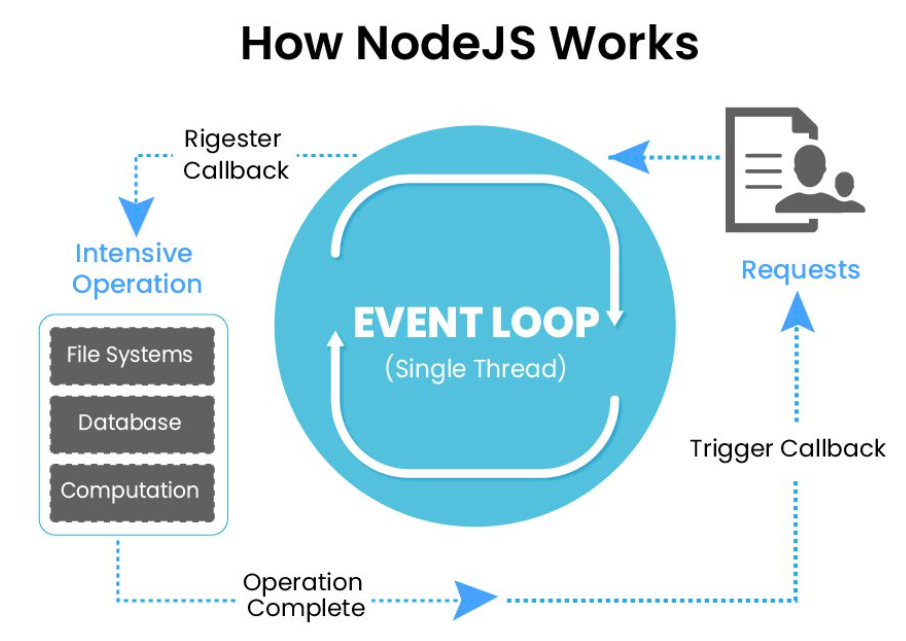
\includegraphics[scale=0.5]{img/NodeJS-work.png}
    \caption{Cách vận hành của NodeJS}
    \label{fig:nodejs}
\end{figure}

Mặc dù Node.js hoạt động trên một luồng duy nhất cho logic ứng dụng của người dùng, nó vẫn sử dụng nhiều luồng ở tầng thấp hơn thông qua thư viện "libuv" để xử lý các hoạt động I/O. Trái tim của Node.js là “event loop”. Đây là vòng lặp sự kiện mà ở đó Node.js tiếp tục lắng nghe sự kiện và thực hiện các hàm gọi lại khi một sự kiện được kích hoạt. Vòng lặp sự kiện cho phép Node.js xử lý hàng nghìn kết nối đồng thời mà không cần phải tạo ra chi phí quản lý luồng. Khi thao tác I/O hoàn tất, hệ điều hành thông báo cho Node.js, và Node.js sau đó thực thi hàm callback tương ứng để xử lý kết quả hoặc tiếp tục xử lý logic.

\subparagraph{Ưu điểm của NodeJS:}
\begin{itemize}
    \item \textbf{Hiệu suất cao:} Nodejs chạy đơn luồng, sử dụng V8 Engine, giúp ứng dụng đảm bảo tốc độ khi có nhiều requests. 
    \item \textbf{Xử lý bất đồng bộ và I/O hướng sự kiện:} Khả năng xử lý I/O bất đồng bộ, giúp Nodejs có thể xử lý nhiều tasks, mà không cần phải chờ kết quả của task trước đó. 
    \item \textbf{Phát triển ứng dụng:} Có thể sử dụng để phát triển ứng dụng ở cả phía client và server. 
    \item \textbf{Module đa dạng:} Nodejs sở hữu một cộng đồng duy trì, phát triển modules, thư viện giúp cho việc phát triển ứng dụng nhanh chóng.
    \item \textbf{Stream và xử lý file lớn:} Nodejs hỗ trợ streaming, cho phép xử lý các file có kích thước lớn không tốn nhiều tài nguyên.
    \item \textbf{Phù hợp với ứng dụng real time:} Do Nodejs xử lý bất đồng bộ, thích hợp với các ứng dụng real time như: chat applications, streaming services,...
    \item \textbf{Hệ sinh thái phong phú}: Với hơn 50,000 gói có sẵn trong Node Package Manager (NPM), các nhà phát triển có thể dễ dàng tìm và sử dụng các thư viện theo nhu cầu của họ mà không cần phải viết lại từ đầu, tiết kiệm đáng kể thời gian và công sức.
    \item \textbf{Tính nhất quán trong mã nguồn}: NodeJS cho phép sử dụng cùng một ngôn ngữ lập trình (JavaScript) cho cả phía máy chủ và máy khách. Điều này không chỉ giúp giảm thiểu sự không đồng bộ giữa client và server mà còn làm cho việc bảo trì và quản lý mã nguồn trở nên dễ dàng hơn.
 
\end{itemize}

Nhược điểm của NodeJS:
\begin{itemize}
    \item Cần có kiến thức nền tảng về JavaScript.
    \item Khá phức tạp trong việc thao tác với cơ sử dữ liệu quan hệ.
    \item Mỗi callback sẽ đi kèm với rất nhiều callback lồng nhau khác, dễ dẫn đến tình trạng "callback hell".
    \item Không phù hợp với các tác vụ đòi hỏi nhiều CPU core.
\end{itemize}

\subsection{ExpressJS}

ExpressJS là một framework được xây dựng trên nền tảng của NodeJS. Nó cung cấp các tính năng mạnh mẽ để phát triển web hoặc mobile. ExpressJS hỗ trợ các method HTTP và middleware tạo ra API vô cùng mạnh mẽ và dễ sử dụng. Với ExpressJS, bạn có thể xây dựng các API RESTful dễ dàng hơn và quản lý dữ liệu hiệu quả mà không cần viết quá nhiều code phức tạp. ExpressJS giúp bạn tập trung vào logic ứng dụng thay vì xử lý chi tiết các yêu cầu HTTP.

ExpressJS tập trung vào công việc tối ưu hóa việc xây dựng web ứng dụng bằng cách cung cấp một cấu trúc hoạt động và chỉ định rõ ràng việc xử lý yêu cầu và phản hồi. Nền tảng cũng hỗ trợ tích hợp các phần mềm trung gian bên ngoài để mở rộng chức năng của ứng dụng. 

\begin{figure}[H]
    \centering
    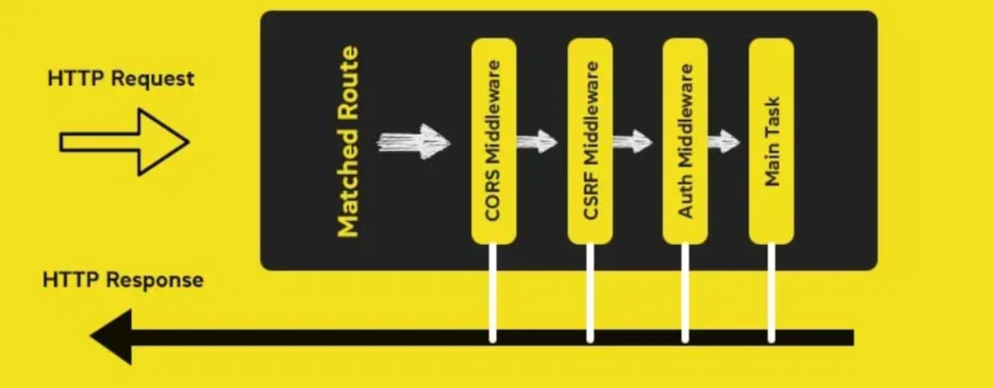
\includegraphics[scale=0.5]{img/ExpressJS-workflow.png}
    \caption{Luồng thực thi của ExpressJS}
    \label{fig:expressjs}
\end{figure}

Express.js hỗ trợ xây dựng API tuân thủ các nguyên tắc của kiến trúc REST (Representational State Transfer) thông qua việc thiết lập các route tương ứng với từng yêu cầu. API này sẽ bao gồm các tính năng như:
\begin{itemize}
    \item Xem danh sách tất cả sản phẩm.
    \item Xem thông tin chi tiết của một sản phẩm.
    \item Thêm một sản phẩm mới.
    \item Cập nhật thông tin sản phẩm.
    \item Xóa sản phẩm.
\end{itemize}

Các tính năng chính của ExpressJS:
\begin{itemize}
    \item \textbf{Định tuyến (Routing)}: cung cấp cơ chế hoạt động cơ bản để xác định điểm cuối và xử lý các yêu cầu HTTP đến từ các công cụ đường dẫn. Công việc quản lý định tuyến giúp xử lý logic yêu cầu riêng biệt cho từng phần của ứng dụng (GET, POST, PUT, DELETE,...), từ đó tạo điều kiện cho việc mở rộng và bảo trì một cách dễ dàng.
    \item \textbf{Middleware}: là hàm đặc biệt cho ExpressJS, cho phép thực thi các thao tác trung gian trước khi yêu cầu đến điểm cuối. Nó cho phép người dùng xác thực, xử lý lỗi, quản lý phiên, nén dữ liệu và nhiều tác vụ khác. 
    \item \textbf{Hỗ trợ công cụ mẫu (Templating Engine)}: hỗ trợ nhiều công cụ mẫu phổ biến nhằm tạo ra các trang HTML động trở nên dễ dàng và linh hoạt. VD: EJS (cho phép nhúng JavaScript trực tiếp vào HTML), Pug (Cung cấp cú pháp ngắn gọn, dễ đọc hơn để tạo HTML), Handlebars và Mustache (sử dụng để quản lý views và tạo HTML)
    \item \textbf{Quản lý tệp và dữ liệu tĩnh}: Middleware express.static() giúp việc phục vụ các tệp tĩnh trong dự án trở nên đơn giản. ExpressJS sẽ tự động xử lý việc cung cấp chúng cho người dùng khi họ yêu cầu.
\end{itemize}

\subsection{MongoDB}
MongoDB là một hệ thống cơ sở dữ liệu phi quan hệ (NoSQL database), mã nguồn mở được phát triển bới MongoDB Inc. Do là một database hướng tài liệu (document), một dạng của NoSQL database, vì thế, MongoDB tránh cấu trúc table-based của relational database để thích ứng với các tài liệu như JSON có schema rất linh hoạt gọi là BSON nên mỗi một collection sẽ các các kích cỡ và các document khác nhau. Các dữ liệu được lưu trữ trong document kiểu JSON nên truy vấn sẽ rất nhanh.

\begin{figure}[htp!]
    \centering
    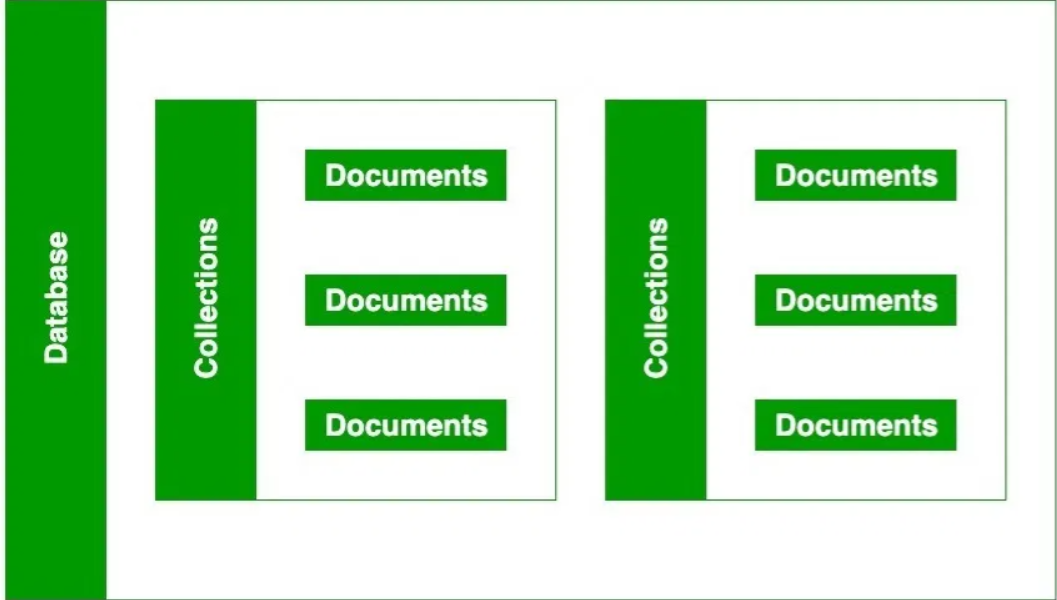
\includegraphics[scale=0.5]{img/MongoDB_work.png}
    \caption{Các thành phần trong MongoDB}
    \label{fig:mongodb}
\end{figure}

MongoDB hỗ trợ tất cả các ngôn ngữ phổ biến như C, C++, C\# và .Net, Go, Java, NodeJS, Perl, PHP, Python, Motor, Ruby, Scala, Swift, Mongoid. Vì vậy, MongoDB đã trở thành một trong những NoSQL database nổi trội nhất bấy giờ, được dùng làm backend cho rất nhiều website như eBay, SourceForge, The New York Times, Facebook, Nokia, eBay, Adobe, Google,... để lưu trữ lượng lớn dữ liệu của họ.

MongoDB không chỉ đơn thuần là một cơ sở dữ liệu, mà còn là một hệ sinh thái hoàn chỉnh với nhiều tính năng và công cụ hỗ trợ. Các tính năng và ưu điểm của MongoDB làm cho việc lưu trữ và xử lý dữ liệu trở nên dễ dàng và hiệu quả hơn, đáp ứng nhu cầu trong nhiều lĩnh vực, đặc biệt là trong Data analyst. Data analyst có thể sử dụng MongoDB để lưu trữ, xử lý và truy vấn các loại dữ liệu khác nhau. Ngoài ra, MongoDB cũng cung cấp các công cụ để truy vấn dữ liệu, tạo báo cáo và thực hiện các phân tích dữ liệu phức tạp cho data analyst. Vì vậy, có thể nói rằng MongoDB là một công cụ hữu ích cho data analyst trong việc lưu trữ và phân tích dữ liệu.

\subparagraph{Các tính năng chính của MongoDB:}
\begin{itemize}
    \item \textbf{Schema-less Database:} giúp tăng tính linh hoạt và giảm thời gian phát triển các ứng dụng, đặc biệt là đối với các ứng dụng có tính chất thay đổi dữ liệu thường xuyên hoặc không có một cấu trúc dữ liệu cố định. Do đó, bạn có thể lưu trữ các tài liệu với các fields và giá trị (values) khác nhau mà không cần tuân theo một cấu trúc cố định và không cần yêu cầu sự định nghĩa trước về cấu trúc của chúng. Tuy nhiên, tính năng này sẽ dẫn đến khó khăn trong việc truy vấn và xử lý dữ liệu nếu không có sự quản lý và thiết kế cẩn thận.
    \item \textbf{Document Oriented:} MongoDB được thiết kế để lưu trữ dữ liệu dưới dạng tài liệu (document). Mỗi tài liệu trong MongoDB được lưu trữ dưới một bản ghi độc lập bao gồm các fields (key-value pair) và giá trị tương ứng.
    \item \textbf{Indexing:} MongoDB tạo ra index để tăng tốc độ truy vấn và tìm kiếm dữ liệu trong cơ sở dữ liệu. Khi truy vấn dữ liệu, MongoDB sử dụng các Index để nhanh chóng tìm kiếm và trả về các tài liệu phù hợp với tiêu chí truy vấn. Việc sử dụng Index giúp giảm thời gian truy vấn tìm kiếm dữ liệu, đồng thời giúp tăng hiệu suất và khả năng mở rộng của MongoDB.
    \item \textbf{Replication:} là quá trình đồng bộ dữ liệu giữa các node trong một cluster MongoDB. Một cluster MongoDB sẽ gồm một node primary và nhiều node secondary. Node primary sẽ chịu trách nhiệm ghi dữ liệu mới vào cơ sở dữ liệu, còn các node secondary chỉ đọc dữ liệu. Với tính năng Replication, MongoDB có khả năng tự động sao lưu dữ liệu, đảm bảo độ tin cậy và khả năng phục hồi của cơ sở dữ liệu, đồng thời giúp tăng khả năng mở rộng của hệ thống.
    \item \textbf{Sao lưu và phục hồi:} MongoDB cung cấp tính năng sao lưu và phục hồi dữ liệu linh hoạt, cho phép lưu trữ các bản sao của dữ liệu và phục hồi dữ liệu trong trường hợp xảy ra sự cố.
    \item \textbf{Bảo mật:} MongoDB hỗ trợ nhiều tính năng bảo mật, bao gồm chứng thực người dùng (user authentication), mã hóa dữ liệu (data encryption) và kiểm soát quyền truy cập (access control).
\end{itemize}

\subsubsection{Ưu điểm của MongoDB:}
\begin{itemize}
    \item \textbf{Linh hoạt:} Do là một hệ thống cơ sở dữ liệu phi quan hệ nên nó cung cấp khả năng lưu trữ dữ liệu bất cứ khi nào, bất cứ nơi đâu, không cần phải tuân thủ một mô hình quan hệ cụ thể.
    \item \textbf{Khả năng mở rộng:} Nhờ tính năng sharding cho phép phân chia dữ liệu thành nhiều phần và lưu trữ trên nhiều máy chủ, nên MongoDB có khả năng mở rộng dễ dàng.
    \item \textbf{Tốc độ truy xuất nhanh:} MongoDB có thể đáp ứng các yêu cầu truy vấn dữ liệu trong thời gian ngắn hơn so với các hệ thống cơ sở dữ liệu quan hệ truyền thống.
    \item \textbf{Tính khả dụng cao:} MongoDB cung cấp tính năng sao lưu và phục hồi dữ liệu, giúp người dùng bảo vệ dữ liệu của mình khỏi những rủi ro.
    \item \textbf{Dễ dùng và tích hợp:} MongoDB cung cấp các công cụ quản lý dữ liệu trực quan và dễ sử dụng, giúp người dùng tối ưu hóa hiệu suất và quản lý cơ sở dữ liệu một cách dễ dàng. Đồng thời, dễ dàng tích hợp với Big Data Hadoop.
\end{itemize}

\subsubsection{Nhược điểm của MongoDB:}
\begin{itemize}
    \item Cần sử dụng bộ nhớ cao để lưu trữ dữ liệu (data storage).
    \item Không được phép lưu trữ hơn 16MB data trong tài liệu (do sử dụng BSON).
    \item Data nesting trong BSON cũng bị hạn chế, bạn không được phép nest data quá 100 cấp độ.
\end{itemize}

\subsubsection{So sánh MongoDB và MySQL:}
\begin{figure}[H]
    \centering
    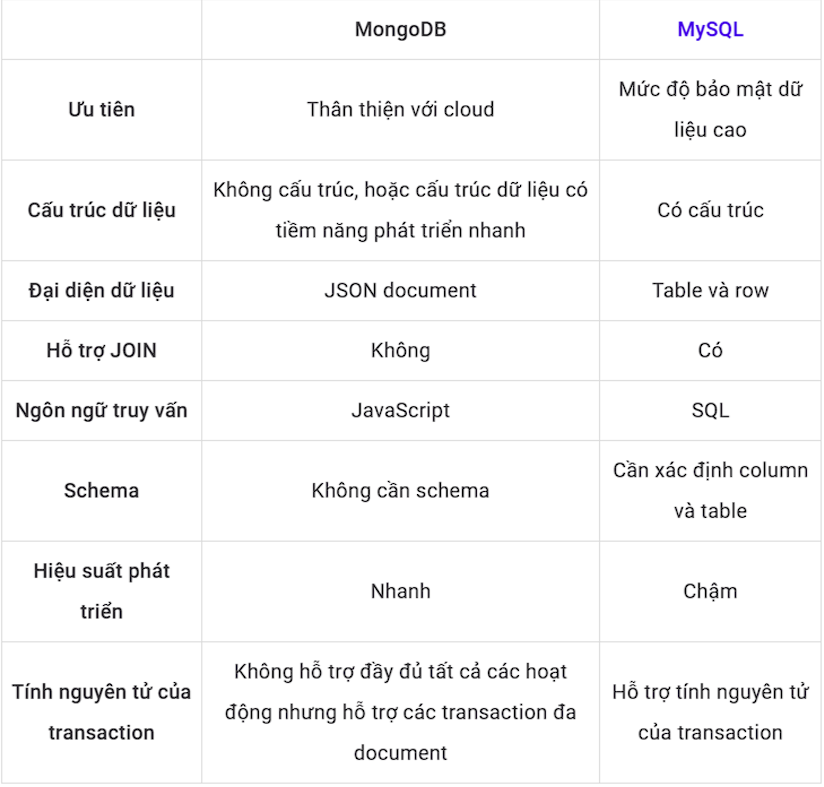
\includegraphics[width=0.8\textwidth]{img/MongoDB_MySQL_comparision.png}
    \caption{So sánh giữa MongoDB và MySQL}
    \label{fig:mongodb_mysql_comparison}
\end{figure}

\section{Phát triển server}
Phát triển server  (máy chủ) là một phần quan trọng trong quá trình xây dựng và triển khai ứng dụng web hoặc hệ thống phần mềm. Nó liên quan đến việc thiết kế, xây dựng, triển khai và duy trì các server - những hệ thống phần cứng hoặc phần mềm chịu trách nhiệm xử lý, lưu trữ và truyền tải dữ liệu giữa người dùng và ứng dụng. Mục tiêu của phát triển server là đảm bảo hệ thống hoạt động ổn định, có khả năng mở rộng và xử lý một lượng lớn yêu cầu từ người dùng.

\subsection{React Server Components (RSC)}
React Server Components (RSC) là một tính năng mới trong React, cho phép các component của React chạy hoàn toàn trên server thay vì trên client. Điều này giúp tối ưu hiệu năng, giảm tải công việc cho client, và tăng tốc độ tải trang.

RSC đặc biệt phù hợp cho các ứng dụng web phức tạp, nơi mà hiệu suất là yếu tố quan trọng. Các ứng dụng như nền tảng thương mại điện tử, ứng dụng truyền thông xã hội, hoặc các ứng dụng cần xử lý lượng dữ liệu lớn từ server sẽ hưởng lợi nhiều từ RSC.

React được tạo ra để kết hợp và áp dụng gia tăng vào các codebases hiện có. RSC mở rộng các nguyên tắc cơ bản của React vượt ra ngoài việc chỉ là một thư viện render, bằng cách tích hợp việc lấy dữ liệu và giao tiếp từ xa giữa client-server trong framework. RSCs tự động lấy dữ liệu và render hoàn toàn trên máy chủ, và kết quả HTML được truyền vào React component tree phía client, xen kẽ với các Server và Client Components khác khi cần thiết. Quá trình này loại bỏ nhu cầu render lại phía client, từ đó cải thiện hiệu suất. Khi một RSC cần được render lại do sự thay đổi trạng thái, nó sẽ làm mới trên server và hợp nhất vào DOM hiện có mà không cần làm mới toàn bộ trang. Kết quả là, trạng thái client được giữ nguyên ngay cả khi các phần của giao diện được cập nhật từ máy chủ.

\subsubsection{Quy trình làm việc khi không có RSC và khi có RSC:}

\begin{figure}[H]
    \centering
    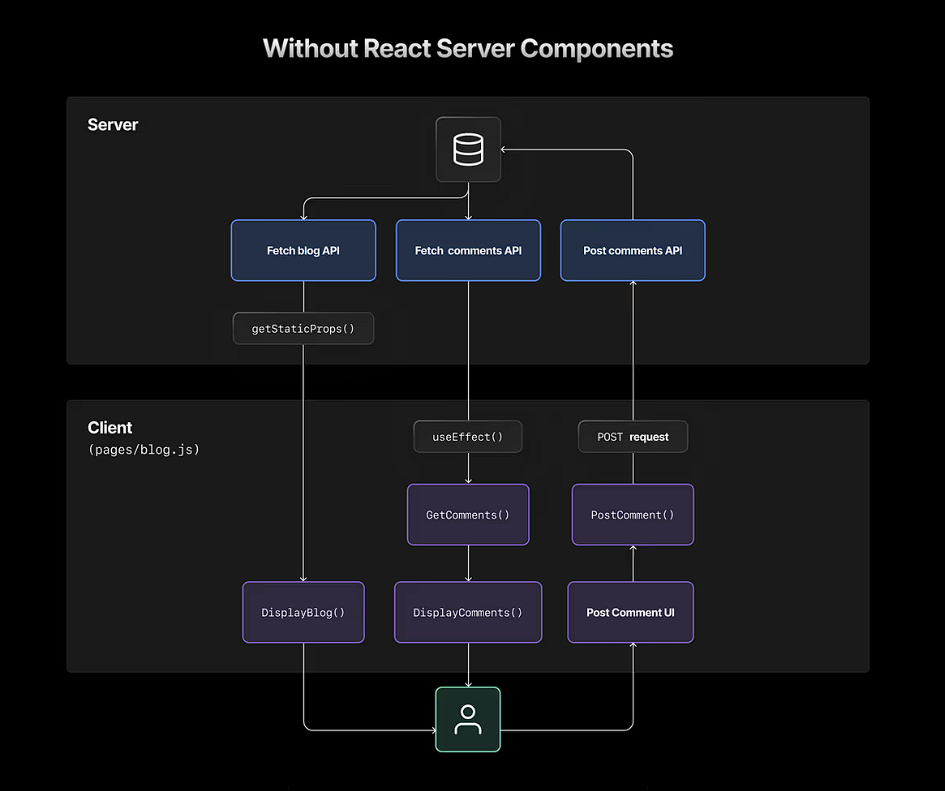
\includegraphics[width=0.8\textwidth]{img/withoutRSCs.png}
    \vspace{0.5cm}
    \caption{Khi không có RSC}
\end{figure}

\begin{figure}[H]
    \centering
    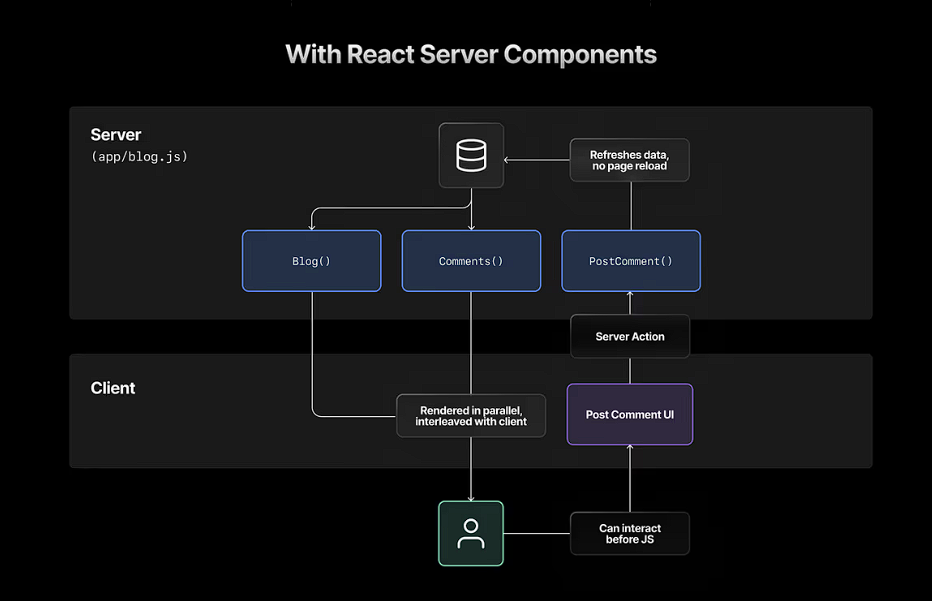
\includegraphics[width=0.8\textwidth]{img/withRSCs.png}
    \vspace{0.5cm}
    \caption{Khi có RSC}
\end{figure}

Như chúng ta có thể thấy, khi không có React Server Component (RSC) thì việc lấy dữ liệu cần thêm một layer API. Còn với khi có thêm React Server Component việc lấy dữ liệu và render giao diện người dùng (UI) có thể được thực hiện từ cùng một component và Server Actions cũng sẽ cung cấp phương pháp giúp cho người dùng có thể tương tác với dữ liệu phía máy chủ trước khi JavaScript tải trên trang. 

\subparagraph{Ưu điểm của React Server Components:}
\begin{itemize}
    \item \textbf{Tăng hiệu suất:} Nhờ vào việc giảm lượng JavaScript cần tải và xử lý trên client.
    \item \textbf{Thân thiện với SEO:} Nội dung được render trên server dễ dàng cho các công cụ tìm kiếm thu thập và lập chỉ mục hơn. 
    \item \textbf{Cải thiện trải nghiệm người dùng}: Tăng tốc độ tải trang và tăng tính tương tác của ứng dụng. 
\end{itemize}

\subsection{Vercel}

Vercel là một cloud platform (nền tảng đám mây) được tạo ra nhằm phục vụ việc phát triển và triển khai ứng dụng web nhanh chóng và dễ dàng. Nền tảng này cho phép bạn xây dựng, triển khai và quản lý các ứng dụng web mà không cần quan tâm đến việc cấu hình hệ thống máy chủ. Vercel hỗ trợ các ứng dụng web được viết bằng nhiều ngôn ngữ lập trình và nhiều framework khác nhau, như JavaScript, TypeScript, Python, Go,.... Với khả năng tự động hóa quá trình triển khai với CI/CD (Continuous Integration/Continuous Deployment), nó giúp các lập trình viên có thể triển khai mã nguồn của mình một cách nhanh chóng chỉ với vài thao tác đơn giản. 

Nó cung cấp 3 tính năng chính: deploy dễ dàng, preview trực tiếp và deliver đến khách hàng nhanh chóng.

\subparagraph{Ưu điểm của Vercel:}
\begin{itemize}
    \item \textbf{Tích hợp với Git:} Khi bạn kết nối tài khoản Github / Gitlab với Vercel, hệ thống sẽ tự động deploy mỗi khi có sự thay đổi trong nhánh chính của repository của bạn. Điều này giúp giảm thời gian triển khai và giảm tải cho bạn. Tích hợp với Git còn giúp cho quá trình phát triển và bảo trì mã nguồn trở nên mượt mà và hiệu quả hơn bởi việc sử dụng các tính năng của Git.
    \item \textbf{Hỗ trợ nhiều ngôn ngữ:} Vercel hỗ trợ nhiều ngôn ngữ lập trình, bao gồm JavaScript, React, Next.js, và nhiều ngôn ngữ khác.
    \item \textbf{Tốc độ nhanh:} Vercel cung cấp tốc độ tải nhanh và độ trễ thấp do có hệ thống phân tán tải nặng rộng rãi trên toàn thế giới, giúp cho trải nghiệm của người dùng tốt hơn.
    \item \textbf{Tích hợp CI/CD:} Vercel cung cấp tích hợp CI/CD (Continuous Integration/Continuous Deployment) mặc định, giúp cho quá trình triển khai và quản lý dự án web trở nên dễ dàng hơn.
    \item \textbf{Hỗ trợ API và serverless functions:} Nền tảng này cũng hỗ trợ việc triển khai các dịch vụ API và serverless functions, giúp bạn xây dựng các ứng dụng phức tạp hơn.
\end{itemize}